\section{Used Models and Images}
\label{sec:data}
% vortrainierte Neural Networks erklären/erwähnen
% alle basieren auf der Image Database "ImageNet"
For the upcoming experiments in section \ref{sec:evaluation} we need to decide which network model we use and which images are feasible as source or \emph{guide image}.
As classification network we chose to use \emph{ResNet}\cite{he2016deep}, shorthand for \emph{Residual Network}, because it is the current state of the art providing the lowest error rate and hence performs best.\cite{cnnComparison}
It offers three variations differing in the layer amount(50, 101, 152).
Due to performance reasons, see section \ref{TODO}, we decided to use the ResNet50.
To apply the \emph{dream} we use a slightly modified version of the original Google deep dream code for the neural network framework caffe\cite{googledeepdream}.

By analyzing various existing \emph{dreamed images}, we came to the conclusion that images with a lot of varying objects offering different features might lead to more interesting results.
Hence we were looking for images containing: 
\begin{itemize}
	\item landscape with varying vegetation
	\item houses
	\item water because it offers a lot of noise to act upon
	\item clouds because of the real-life relatability mentioned in section \ref{sec:visual-aspects}
\end{itemize}

To find images with these properties we used \emph{Flickr} because it allows to search for images that are licensed under the \emph{creative commons}.
Figure \ref{fig:imgbeestemarkt} is an image of the Beestenmarkt in Leiden and offers three of the wanted features: water, clouds and buildings.
In addition to that a few people are also present in the picture who might be transformed as well.
The second image, visible in figure \ref{fig:imgfield}, is a closeup of some vegetation on a field offering a lot of small distinctive features.
It contains two of the features we are looking for, namely a landscape with varying vegetation and clouds. It is also advantageous that the grass land in the background is made up of different colors ranging from green to yellow to almost brownish.
The third image, portrayed in figure \ref{fig:imglandscape}, is similar to the second one. Yet it offers different wanted features because it includes small houses, a forest and only one huge cloud.

%TODO: Hier erwähnen welches  verwendet wird und wie viele Layer es hat


\begin{figure}[H]
	\minipage{0.32\textwidth}
	\centering
	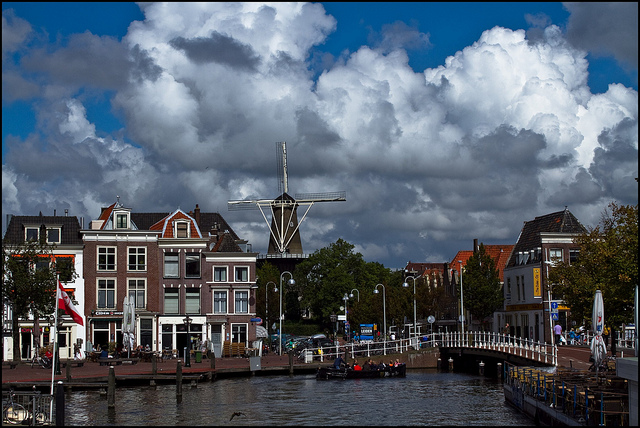
\includegraphics[width=1\linewidth]{img/beestemarkt.jpg}
	\caption{Source image displaying the Beestemarkt in Leiden\cite{imgbeestemarkt}.}
	\label{fig:imgbeestemarkt}
	\endminipage\hfill
	\minipage{0.32\textwidth}
	\centering
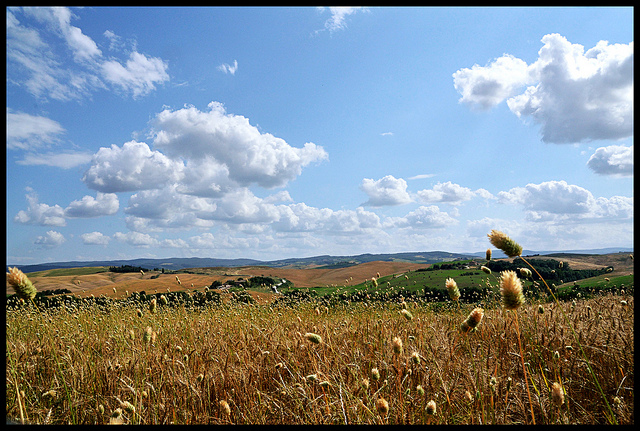
\includegraphics[width=1\linewidth]{img/field.jpg}
\caption{Source image portraying a field with mountains in the background\cite{imgfield}.}
\label{fig:imgfield}
\endminipage\hfill
\minipage{0.32\textwidth}
\centering
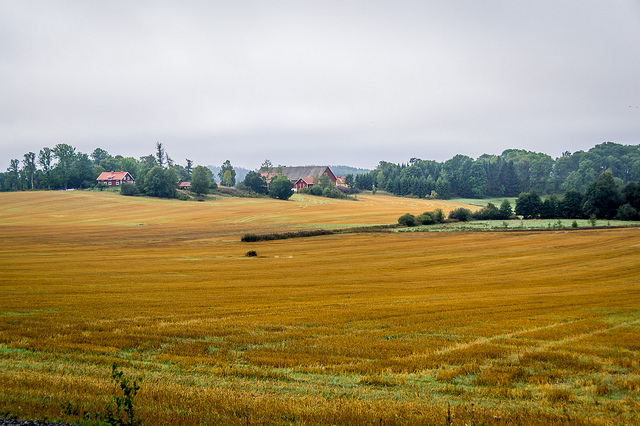
\includegraphics[width=1\linewidth]{img/landscape.jpg}
\caption{Source image portraying a landscape with a small houses and trees\cite{imglandscape}.}
\label{fig:imglandscape}
\endminipage\hfill
\end{figure}